\documentclass[template.tex]{subfiles}

\usepackage{comment} 

\begin{document}

 %% \ SECTION 2
\section{The Phydra package: structure \& features} \label{Section:phydrapackage}
% 2nd Section:
% Background, theoretical framework. Specifics here!
\begin{comment}
Andrew's comments: (THIS IS METHODS)
- describe modelling framework and details how you built everything
- now explain in detail what the package is \& can do, what the structure is like
- clarify that it is situated in complexity between custom scripts and modelling tools with graphical interfaces. It would be possible to design a graphical interface for this later on, but that is not the target audience.


"Python is a high-level programming language well suited to rapid development and prototyping, as well as being more accessible to domain scientists than low-level languages such as FORTRAN or C++." - Mobius GMD paper
- This is also due to the dynamic interpretation of python, which makes python slower, but python is rapidly developing and leveraging other lower level language for speed. Also has high functionality for parallelisation of code execution which is very relevant to complex marine ecosystem models. 

- clearly state limitations (scope) of phydra 
- mention that xarray-simlab is general enough to support IBMs! But not developed here.
\end{comment}

The Phydra package is an open-source project, that would be impossible without the previous efforts of other developers. Two relatively young packages, which are currently still being developed, \cite{Bovy2018Xarray-simlab:Interactively} and \cite{Beal2018GEKKOSuite}



\subsection{Xarray-simlab: object-oriented modelling framework}
- Further detail on the xarray-simlab framework used for phydra!

"xarray-simlab is a Python library that provides both a generic framework for building computational models in a modular fashion and a xarray extension for setting and running simulations using the xarray.Dataset structure. It is designed for fast, interactive and exploratory modelling."

"xarray-simlab is a tool for fast model development and easy, interactive model exploration. It aims at empowering scientists to do better research in less time, collaborate efficiently and make new discoveries."

specific version used here: v0.4.1 \cite{benoit_bovy_2020_3755979}


The xarray-simlab framework is built on a very few concepts that allow great flexibility in model customisation:

- models
- processes
- variables

\subsubsection{Processes}
in xarray-simlab, (almost) everything is a process.
- in the following sections, introduce the specific implementation of xarray-simlab processes within phydra, what is actually implemented in v1 and how it can be modified and used.


\subsection{GEKKO Optimization suite: compiled solver back end}

"The GEKKO Python package solves large-scale mixed-integer and differential algebraic equations with nonlinear programming solvers. Modes of operation include machine learning, data reconciliation, real-time optimization, dynamic simulation, and nonlinear model predictive control." \cite{Beal2018GekkoSuite}

specific version used here: v0.2.7

\subsubsection{Gekko variable types}
there are more, Gekko is much more complex than our use case, but the ones used in this implementation are
- Parameters. 
- Intermediates. 
- State Variables.  
- Equations.
additionally some functions like summing of terms (sum(x)) or calculating the Euler exponent (exp(x)) have specific implementations as part of the Gekko model syntax.


\subsection{phydra package}
- phydra: easy to use, open source, easy to modify, toolbox
- uses xarray-simlab processes for ALL components (for now, check again)

\subsubsection{Phydra environments} \label{Section:PhysicalEnvironment}

- Forcing can affect one Flow, but can also affect many others, if they are related to the physical environment. This might require a additional fluxes groups defined in the components. 
- explain this here, and present what is included in phydra v1, and how the boilerplate (base classes) can be modified to create your own.
-This describes generalised mixing fluxes for nutrients and other components and provides an interface for model forcing. 
- These are aggregated via xs.group, and individual parameterisations are also possible by an EnvPar object passed in model initiation.

\subsubsection{Components}
- Components are state variables, make sure to use clear wording and explain well

\subsubsection{Flows}
- Flows are parts of differential equations, that affect one or more components, and can be influenced by forcing and the physical environment


\subsection{Model development workflow}

% CONDA NAME DROP
Since python is a fast developing language, we will provide instructions to install a fully compatible virtual environment with the Conda package manager, speparate from a users normal python environment. We recommend to follow the instructions on the Github repository, so that updates in dependent packages do not break the code execution of Phydra. For interactive coding and rapid prototyping we recommend using the jupyter environment that is available via Conda. For more complex and larger model runs on clusters however, python scripts are preferable.

\subsubsection{Dimensionality}
- Dimensionality is a very important fact of building models, and xarray-simlab provides a simple, but sometimes tricky interface for managing dimensionality, so make sure to explain it relatively well here, as well as the implementations.
- I can cite https://www.biogeosciences.net/17/609/2020/ to explain why dimensionality is an important consideration in phytoplankton models.

\subsubsection{Runtime}
- explain what the options are to run the model, depends on if a time implicit method will be added to solve, or if it will just remain with the time explicit steps of xarray-simlab

\subsubsection{Model Diagnostics}
- this is a relevant section, *if* Benoît can help me with creating the ODE visualisation & model diagnostics.

\subsubsection{Parameter fitting}
- this is a relevant section, if i manage to get some decent parameter fitting results for the example 1 and 3.. either only 3 or both, is my feeling. 


\subsection{Forcing (and verification) data} \label{Section:ForcingSection}

To simplify models of complex systems larger processes are not mechanistically implemented, but instead empirically represented as an external forcing. In two of the presented use cases, we adapt a slab representation of ocean physics as defined by \citet{Evans1985ACycles}. The multi-dimensional ocean is reduced to two layers, where the upper layer provides a zero dimensional setting for our ecosystem model. The bottom layer is often assumed to contain a fixed concentration of nutrients (usually nitrate), but this can also vary with depth or time. There is constant exchange between the layers. Nutrients are usually mixing up into the upper layer, where they are consumed by phytoplankton. 

The fraction of all ecosystem components sinking to the bottom layer are lost from the system. These exchanges of water masses within this two-layered model ocean are driven by the empirically derived mixed layer depth (MLD). Additional common forcings that are used in slab models modify phytoplankton growth, e.g. metabolic rates via temperature and light harvesting via irradiance. Such forcing can situate a slab model a theoretically in any location in the global ocean. Compared to the natural habitat of marine plankton, the slab model is a radical simplification. With the appropriate forcing the resulting simulations can yield meaningful results that can be compared with bulk properties of the marine ecosystem \cite[e.g.][]{Evans1985ACycles, Fasham1990a}. 
\subsection{Forcing (and verification) data} \label{Section:ForcingSection}

To simplify models of complex systems larger processes are not mechanistically implemented, but instead empirically represented as an external forcing. In two of the presented use cases, we adapt a slab representation of ocean physics as defined by \citet{Evans1985ACycles}. The multi-dimensional ocean is reduced to two layers, where the upper layer provides a zero dimensional setting for our ecosystem model. The bottom layer is often assumed to contain a fixed concentration of nutrients (usually nitrate), but this can also vary with depth or time. There is constant exchange between the layers. Nutrients are usually mixing up into the upper layer, where they are consumed by phytoplankton. 

The fraction of all ecosystem components sinking to the bottom layer are lost from the system. These exchanges of water masses within this two-layered model ocean are driven by the empirically derived mixed layer depth (MLD). Additional common forcings that are used in slab models modify phytoplankton growth, e.g. metabolic rates via temperature and light harvesting via irradiance. Such forcing can situate a slab model a theoretically in any location in the global ocean. Compared to the natural habitat of marine plankton, the slab model is a radical simplification. With the appropriate forcing the resulting simulations can yield meaningful results that can be compared with bulk properties of the marine ecosystem \cite[e.g.][]{Evans1985ACycles, Fasham1990a}. 

\subsection{Modification and further development}

- Similar to how a forcing process can easily be subclassed to supply a different forcing, other processes in xsimlab can be easily subclassed and modified to have a different function, as long as the interaction between state variables matches
- Explain interface to process subclasses, and how it is relatively easy to set up xsimlab processes with slightly different  formulations, but the same basic interaction

% OPEN SOURCE CONTRIBUTION 

Phydra (like Xarray-Simlab and GEKKO) is an open-source project. Contributions are welcome, and they are greatly appreciated. You can contribute in many ways by reporting bugs, submitting feedback, contributing to the development of the code or the documentation for example. See the contributing guidelines on the Github repository for further details.







%%% TWO-COLUMN FIGURES
%
%%f
\begin{figure*}[t]
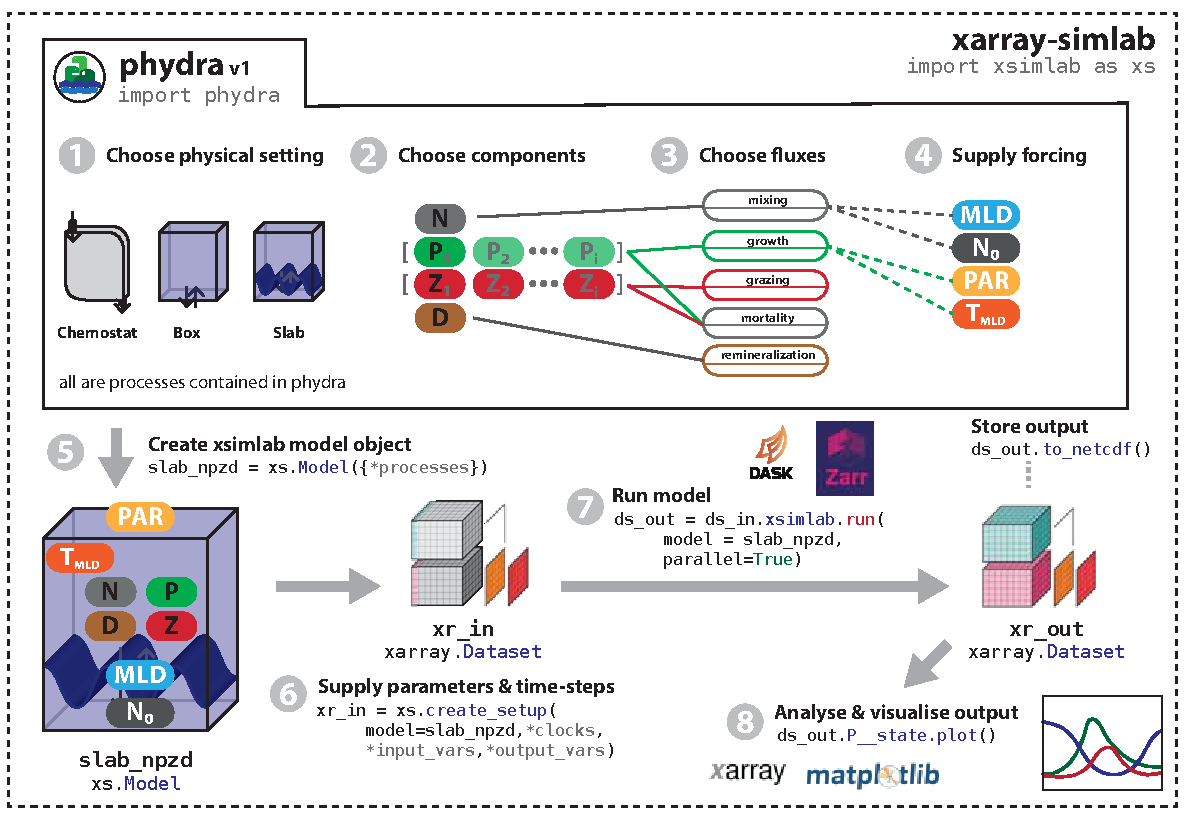
\includegraphics[width=12cm]{Figures/firstdraft_schematics/01__schematics_phydra_1.pdf}
\caption{The phydra package is embedded within the xarray-simlab framework. phydra contains a library of physical settings (1), components (i.e. state variables) (2), fluxes (3) and forcing variables (4), that can be combined and reused to create an xarray-simlab model instance. Xarray-simlab provides the functionality to define the model (5) from processes in the phydra library, supply parameters and create an xarray input (6), then run the model (7) and the resulting output is dynamically stored in another xarray, with fully labelled dimensions and containing all parameters.}
\label{Figure:phydraschematics}
\end{figure*}

general explanation, and then go into detail below (see Figure \ref{Figure:phydraschematics})





% Everything below here is optional, it depends on what I can actually do in the package
% this is a custom function to be able to see references when rendering subfiles:
\biblio

\end{document}